\chapter{Heat Generation and Transport in the Core}
\label{ch:thermal}

Reactivity feedback acts through temperature, so we must know how fission power
becomes temperature. This chapter follows the heat from its birth in the fuel,
across the gap and cladding, to the coolant, and reduces the chain to the lumped
thermal models used in stability analysis.

\section{The path of the heat}

Almost all fission energy---the kinetic energy of the fragments---is deposited in
the fuel pellet within micrometres of the fission event. From there it must
travel: by \emph{conduction} through the ceramic fuel, across the (often
gas-filled) \emph{gap} between pellet and cladding, through the metal
\emph{cladding}, and finally by \emph{convection} into the flowing coolant, which
carries it out of the core to the steam generators or directly to the turbine.
Each step imposes a temperature drop, and the sum of these drops sets the fuel
centreline temperature for a given power.

\begin{figure}[H]
\centering
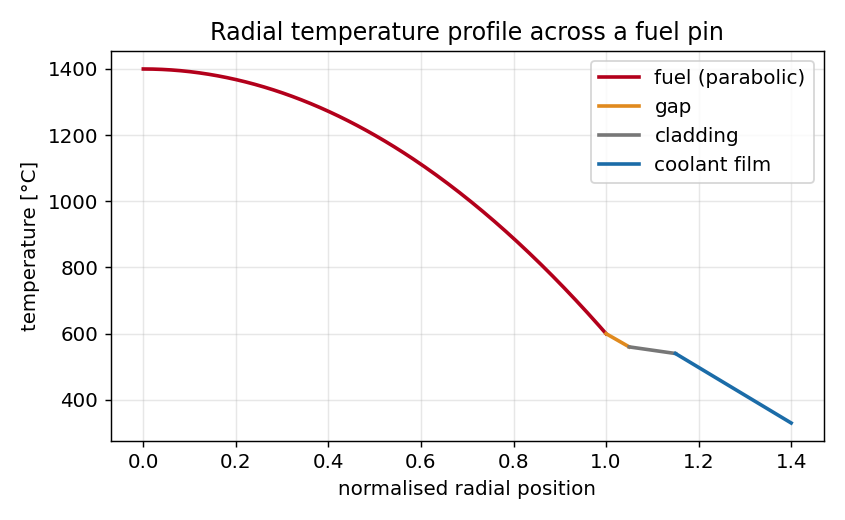
\includegraphics[width=0.74\linewidth]{figures/fuelT.png}
\caption{Schematic radial temperature profile across a fuel pin. The largest drop
is the parabolic profile within the low-conductivity ceramic fuel; further drops
occur across the gap, cladding, and coolant film. The fuel centreline runs
hottest and responds essentially instantly to power changes---the basis of prompt
Doppler feedback.}
\label{fig:fuelT}
\end{figure}

\section{Conduction in the fuel pellet}

For a cylindrical fuel pin with uniform volumetric heat generation $q'''$ and
constant conductivity $k_f$, the steady radial conduction equation
\begin{equation}
\frac{1}{r}\frac{\dd}{\dd r}\!\left(r\,k_f\frac{\dd T}{\dd r}\right) + q''' = 0
\end{equation}
integrates to the parabolic profile
\begin{equation}
T(r) = T_s + \frac{q'''}{4k_f}\!\left(R^2 - r^2\right),
\end{equation}
so the centreline-to-surface temperature rise is
\begin{equation}
\Delta T_{\text{fuel}} = T_c - T_s = \frac{q'''R^2}{4k_f} = \frac{q'}{4\pi k_f},
\end{equation}
where $q'=q'''\pi R^2$ is the linear heat rate (W/m). Remarkably, this rise
depends only on the linear heat rate and the conductivity, not on the pin radius.
Because $\mathrm{UO_2}$ has a low and temperature-dependent conductivity
($k_f$ falls from $\sim 8\unit{W/(m\,K)}$ near room temperature to
$\sim 2\unit{W/(m\,K)}$ at operating temperature), the centreline runs very hot,
often above $1000\degC$ at rated power, even when the surface is near the coolant
temperature. The integral conductivity $\int k_f\,\dd T$ is the natural variable
and is tabulated for fuel design.

\section{Gap, cladding, and film}

Across the pellet--clad gap, heat crosses by conduction through the fill gas and
by radiation; the effective gap conductance $h_g$ depends sensitively on the gap
width, gas composition (helium fill, fission-gas dilution), and burnup. The drop
is $\Delta T_g = q'/(2\pi R\, h_g)$. Conduction through the thin metal cladding
adds a small drop. Finally, convection into the coolant follows Newton's law of
cooling with a heat-transfer coefficient $h$,
\begin{equation}
\Delta T_{\text{film}} = \frac{q'}{2\pi R_{co}\, h},
\end{equation}
where $h$ is obtained from correlations (Dittus--Boelter for single-phase forced
convection; more elaborate correlations in boiling). The total drop from
centreline to bulk coolant is the sum of all four contributions.

\section{The decisive timescales}

For dynamics, the \emph{rates} of temperature change matter as much as the steady
drops. The fuel has a thermal time constant
\begin{equation}
\tau_f = \frac{m_f c_{p,f}}{h_{\text{eff}}A},
\end{equation}
typically a few seconds, after which it equilibrates with the coolant for a given
power. But the \emph{centreline} responds to a power change essentially
instantly---within the conduction time across the pellet---which is why Doppler
feedback (which depends on fuel temperature) is treated as prompt. The coolant
has its own transport time, the time for fluid to traverse the core, of order a
second; moderator and coolant feedback therefore lag the power by this transport
delay. These differing lags---prompt fuel, delayed coolant---are central to
stability: a fast \emph{negative} fuel feedback can stabilise a transient that a
delayed coolant feedback could not catch in time.

\keypoint{The fuel temperature responds promptly to power; the coolant
temperature and void respond with a transport delay. Prompt negative feedback
(Doppler) is the reactor's first and fastest line of defence in a fast
transient; delayed feedback governs the slower stability of the operating point.}

\section{Lumped thermal models for dynamics}

Full thermal-hydraulics is a field in itself, but stability analysis usually uses
\emph{lumped} models that capture the essential dynamics with a few ordinary
differential equations. A widely used two-node model treats the fuel and coolant
as single nodes with temperatures $\Tf$ and $\Tc$:
\begin{align}
m_f c_f \frac{\dd \Tf}{\dd t} &= P(t) - U\!A\,(\Tf - \Tc),\\
m_c c_c \frac{\dd \Tc}{\dd t} &= U\!A\,(\Tf - \Tc) - 2\dot m c_c (\Tc - T_{in}),
\end{align}
where $P$ is the power deposited in the fuel, $U\!A$ the fuel-to-coolant
conductance, $\dot m$ the coolant mass flow, and $T_{in}$ the inlet temperature.
The factor of two in the last term arises from taking the node temperature as the
average of inlet and outlet. Even simpler is the \emph{adiabatic} model used in
fast-excursion analysis, in which heat removal is neglected on the (short)
excursion timescale and the fuel simply integrates the power:
\begin{equation}
C\frac{\dd \Tf}{\dd t} = P(t),
\label{eq:adiabatic}
\end{equation}
with $C$ the fuel heat capacity. This is the model behind the Nordheim--Fuchs
analysis of Chapter~\ref{ch:nonlinear} and the feedback demonstrations of
Chapter~\ref{ch:comp}. Its virtue is that, in the seconds of a prompt excursion,
it is also physically accurate: there simply is not time to remove the heat.

These lumped temperatures are the inputs to the feedback coefficients of the next
chapter. Their dynamics---how fast $\Tf$ and $\Tc$ track power---combine with the
\emph{signs} of the feedback coefficients to determine whether the closed loop is
stable.



\section{Exact conduction in the fuel pin}
\label{sec:fuel-conduction}

\paragraph{Integral conductivity.}
With temperature-dependent $k_f$, define $\theta(T)=\int_{T_{\mathrm{ref}}}^{T}
k_f(T')\dd T'$. Integrating the steady equation
$\frac1r\frac{\dd}{\dd r}(r k_f\,T')+q'''=0$ once gives
$k_f\,\dd T=-(q'''/2)\,r\,\dd r$, hence
\begin{equation}
\theta(T_c)-\theta(T_s)=\frac{q''' R^2}{4}=\frac{q'}{4\pi},
\label{eq:integral-cond}
\end{equation}
\emph{independently of the form of} $k_f(T)$: it is the integral conductivity, not
the temperature, that is linear in the linear heat rate $q'$.

\paragraph{Exact transient solution.}
The homogeneous cylindrical heat equation
$\partial_t T=\kappa(\partial_{rr}T+r^{-1}\partial_r T)$, $\kappa=k_f/(\rho c_p)$,
with $T(R,t)=T_s$, $\partial_rT(0,t)=0$, separates as $T-T_s=\mathcal R(r)e^{-\kappa\nu^2t}$
with $\mathcal R''+\mathcal R'/r+\nu^2\mathcal R=0$, regular solution $J_0(\nu r)$.
The condition $J_0(\nu R)=0$ quantises $\nu_n=\alpha_n/R$ ($J_0(\alpha_n)=0$;
$\alpha_1\approx2.405$), giving
\begin{equation}
T(r,t)-T_s=\sum_{n=1}^{\infty}A_n J_0\!\Big(\frac{\alpha_n r}{R}\Big)
\exp\!\Big(-\frac{\kappa\alpha_n^2}{R^2}t\Big),
\label{eq:bessel-series}
\end{equation}
with $A_n$ from the orthogonality
$\int_0^R J_0(\tfrac{\alpha_n r}{R})J_0(\tfrac{\alpha_m r}{R})r\,\dd r
=\tfrac12 R^2 J_1(\alpha_n)^2\delta_{nm}$.

\begin{proposition}[Fundamental thermal time constant]
\label{prop:thermal-tau}
For $t\gtrsim R^2/\kappa$ the series \eqref{eq:bessel-series} is dominated by $n=1$,
so the fuel relaxes as a single exponential with
\begin{equation}
\tau_f=\frac{R^2}{\kappa\,\alpha_1^2}=\frac{\rho c_p R^2}{k_f\,\alpha_1^2}
\approx\frac{\rho c_p R^2}{5.78\,k_f}.
\end{equation}
\end{proposition}
\begin{proof}
Mode $n$ decays at $\kappa\alpha_n^2/R^2$, increasing in $n$; the ratio of mode $2$
to mode $1$ is $e^{-\kappa(\alpha_2^2-\alpha_1^2)t/R^2}\to0$, leaving the $n=1$
rate $\kappa\alpha_1^2/R^2$, i.e.\ $\tau_f=R^2/(\kappa\alpha_1^2)$,
$\alpha_1^2\approx5.78$.
\end{proof}

\paragraph{The Biot number.}
With $\mathrm{Bi}=hR/k_f$ comparing conduction to convection resistance, the
lumped balance $\rho c_p V\,\dd T/\dd t=-hA(T-T_\infty)$ (decay constant
$\tau=\rho c_p V/(hA)$) is valid for $\mathrm{Bi}\ll1$; for $\mathrm{Bi}\gtrsim1$,
typical of ceramic fuel, the distributed solution \eqref{eq:bessel-series} and
Proposition~\ref{prop:thermal-tau} are required.

\section{Spectral analysis of the two-node thermal model}
\label{sec:twonode-spectral}

Linearising the two-node model about steady state gives $\dot{\boldsymbol\delta}
=\mathbf B\boldsymbol\delta$ for $(\delta\Tf,\delta\Tc)$ with
\begin{equation}
\mathbf B=
\begin{pmatrix}
-\dfrac{U\!A}{m_fc_f} & \dfrac{U\!A}{m_fc_f}\\[6pt]
\dfrac{U\!A}{m_cc_c} & -\dfrac{U\!A+2\dot m c_c}{m_cc_c}
\end{pmatrix}.
\end{equation}
Here $\operatorname{tr}\mathbf B<0$ and
$\det\mathbf B=\dfrac{U\!A\cdot 2\dot m c_c}{m_fc_f\,m_cc_c}>0$, so by the $n=2$
Routh--Hurwitz conditions (Theorem~\ref{thm:rh}) both eigenvalues
\begin{equation}
\lambda_\pm=\tfrac12\Big(\operatorname{tr}\mathbf B\pm
\sqrt{\operatorname{tr}^2\mathbf B-4\det\mathbf B}\Big)
\end{equation}
lie in the left half-plane: the passive thermal network is unconditionally stable.
The constants $\tau_\pm=-1/\lambda_\pm$ are the fast (fuel) and slow (coolant)
lags entering the feedback transfer function $H(s)$ of Chapter~\ref{ch:linear}.
Instability can thus enter only through the neutronic coupling and the sign of the
reactivity feedback, never through the thermal network itself.


\section*{Exercises}
\addcontentsline{toc}{section}{Exercises}
\begin{enumerate}[leftmargin=*,itemsep=2pt]
\item Show that the fuel centreline-to-surface temperature rise depends only on the linear heat rate and conductivity, not the pin radius.
\item List the four temperature drops from fuel centreline to bulk coolant and identify which is usually largest.
\item Explain why Doppler feedback is treated as prompt while moderator feedback is delayed.
\item Justify the adiabatic fuel model \eqref{eq:adiabatic} for analysing a prompt excursion.
\item Estimate the fuel thermal time constant given plausible values and discuss its role in stability.
\end{enumerate}
